\subsection{Matrix dimension L=2}

OBS! Need an number of MC cycles necessary!

All calculations in this subsection are at T = 1.0 K. 

\begin{table}\caption{This table compares the analytical values for L=2 with the numerical ones after $10^6$ Monte Carlo cycles. The values are in units per spin.}\label{tab:compare_values}
\begin{tabular}{ccc}
& Numerical: & Analytical:\\ \hline
$\left<E\right>$ &   -1.9958 & -1.9960\\
$\left<E^2\right>$ &   15.9664 & 15.9679\\
$\left<M\right>$ &    0.0451 & 0\\
$\left<M^2\right>$ &    3.9930 & 3.9933\\
$\left<|M|\right>$ &    0.9986 & 0.9987\\
$\chi$ &   3.9849 & 3.9933\\
  $C_V$& 0.0335 & 0.0321\\
\end{tabular}
\end{table}

\begin{figure}[H]
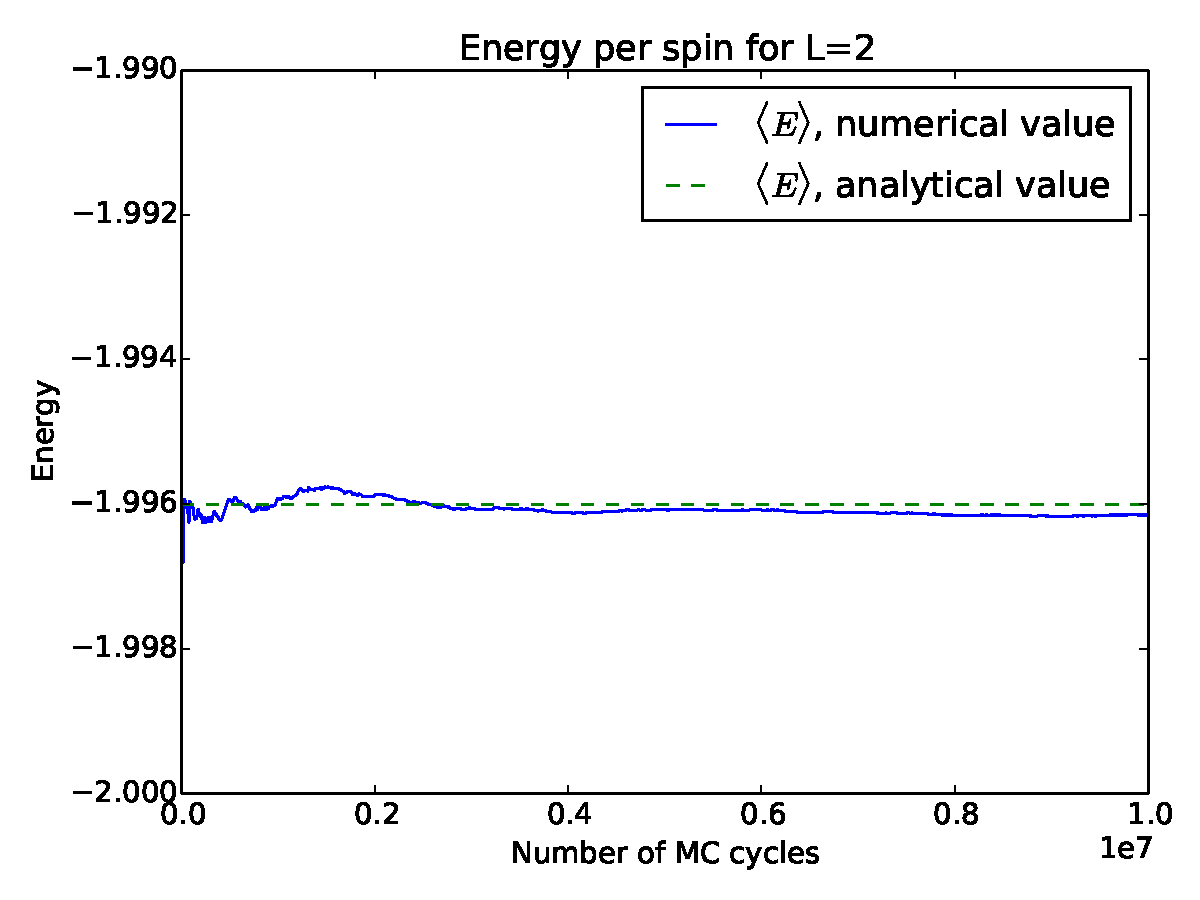
\includegraphics[width=\linewidth]{../results/4b/L_2_energy}\caption{This is a plot of the expectation value of the energy per spin verus number of Monte Carlo cycles. The plot shows that we have a good agreement after $ 5 \cdot 10^{5} $ MC cycles.}\label{fig:L_2_energy}
\end{figure}

\begin{figure}[H]
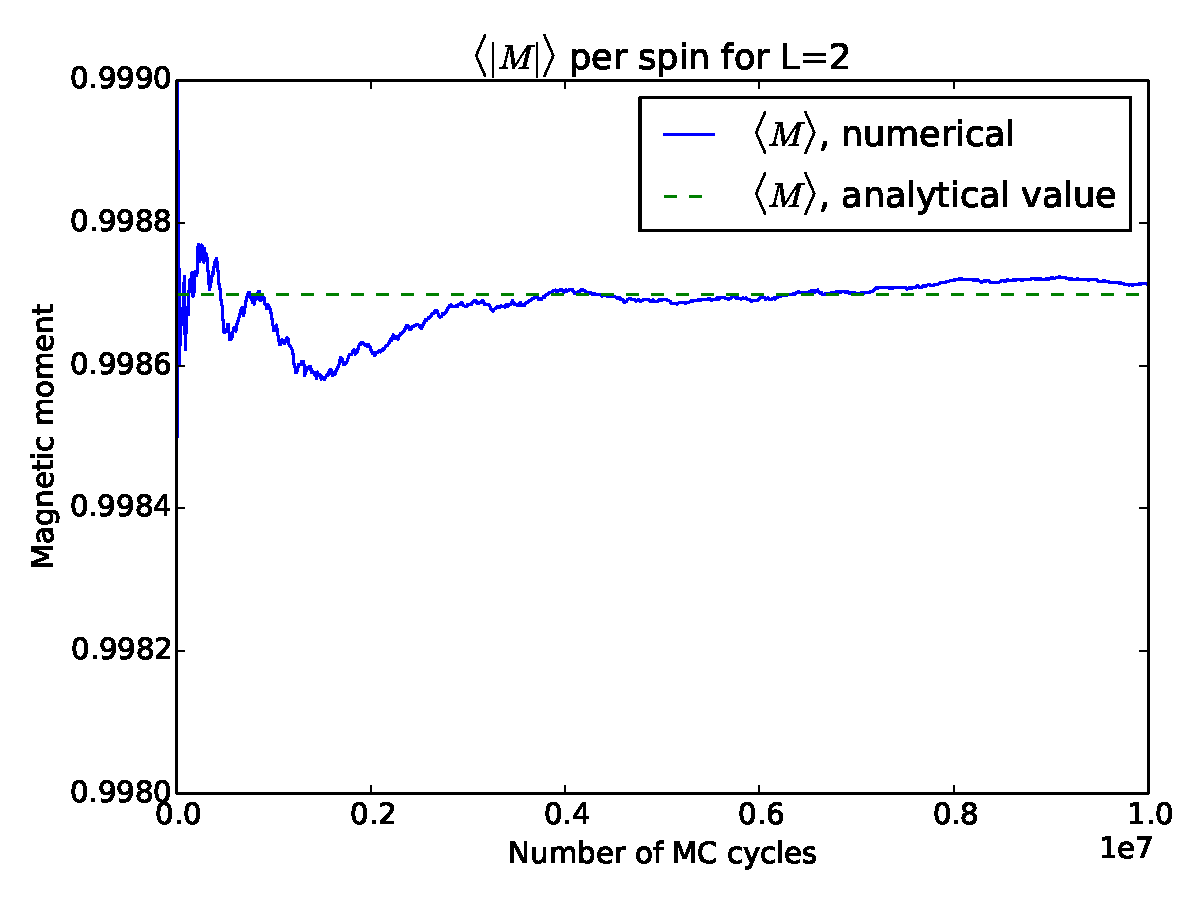
\includegraphics[width=\linewidth]{../results/4b/L_2_magnetic_abs}\caption{This is a plot of the expectation value of the mean absolute value of the magnetic moment per spin verus number of Monte Carlo cycles. The plot shows that we have a good agreement after $ 5 \cdot 10^{5} $ MC cycles.}\label{fig:L_2_magnetic_abs}
\end{figure}

\begin{figure}[H]
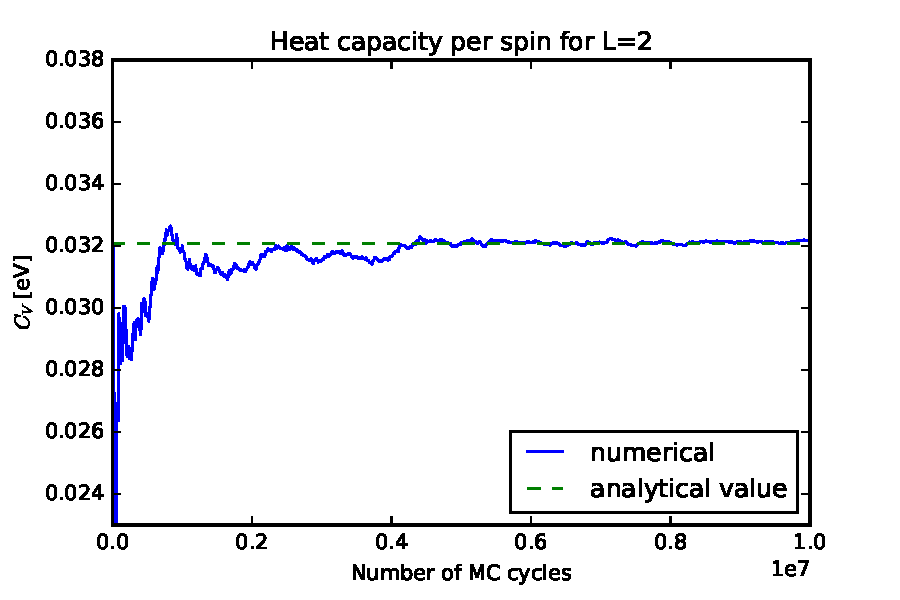
\includegraphics[width=\linewidth]{../results/4b/L_2_heat_capasity}\caption{This is a plot of the heat capacity per spin verus number of Monte Carlo cycles. The plot shows that we have a good agreement after $ 5 \cdot 10^{5} $ MC cycles.}\label{fig:L_2_heat_capacity}
\end{figure}

\begin{figure}[H]
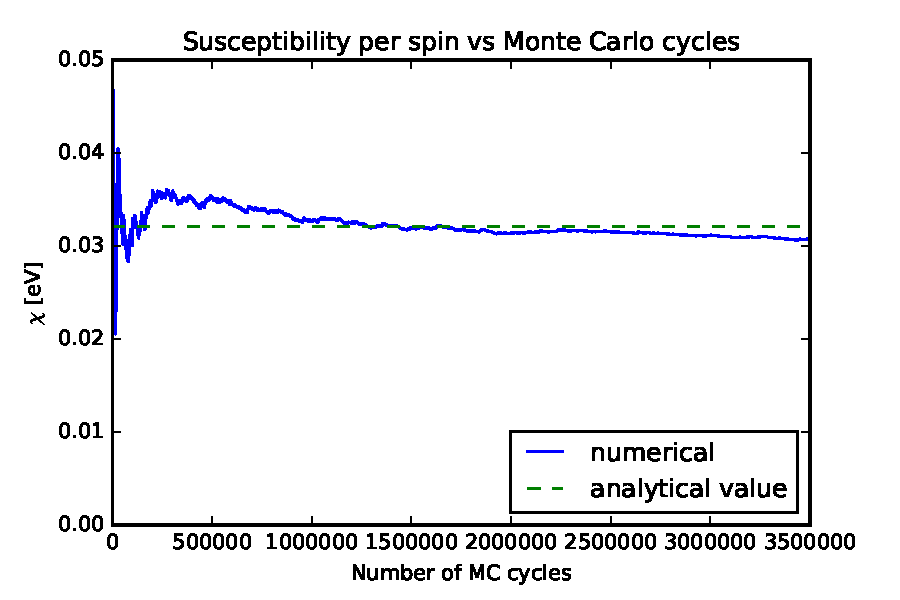
\includegraphics[width=\linewidth]{../results/4b/L_2_susceptibility}\caption{This is a plot of the susceptibility per spin verus number of Monte Carlo cycles. The plot shows that we have a good agreement after $ 5 \cdot 10^{5} $ MC cycles.}\label{fig:L_2_susceptibility}
\end{figure}

\subsection{Matrix dimension L = 20}

HMM: Should define an area that is enough for equilibrium!

OBS: Need the number of MC cycles to reach equilibrium!

OBS: Need equilibration time! (5 1e5?)

OBS: Comment accepted configs T dependency

\subsubsection{Different temperatures}
\begin{figure}[H]
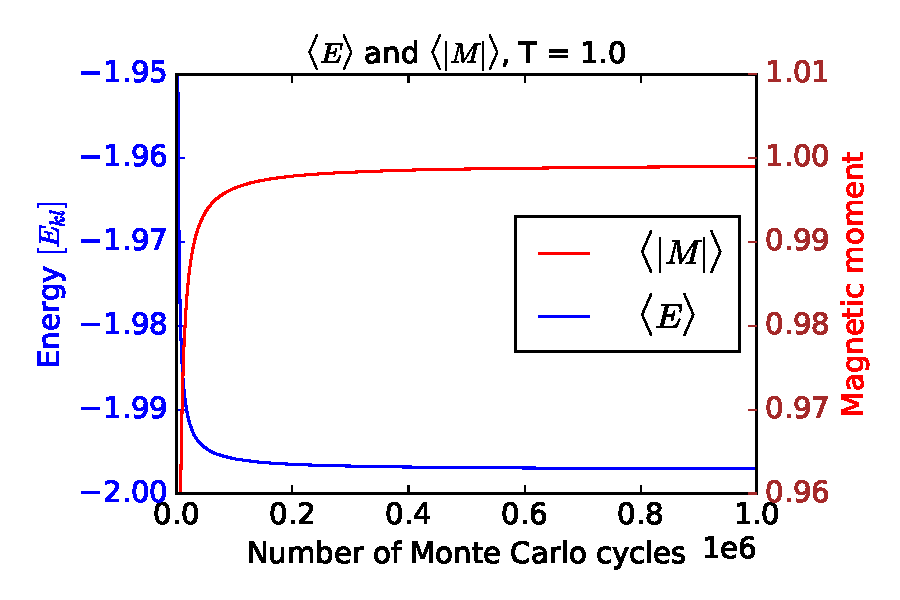
\includegraphics[width=\linewidth]{../results/4c/En_mag_T1_0}\caption{This is a plot of both the expectation value of the energy and absolute magnetic moment per spin verus number of Monte Carlo cycles at T = 1.0 K. The plot shows that an equilibrium is reached already at $2 \cdot 10^{5}$ MC cycles.}\label{fig:L_20_energy_mag_T_1.0}
\end{figure}

\begin{figure}[H]
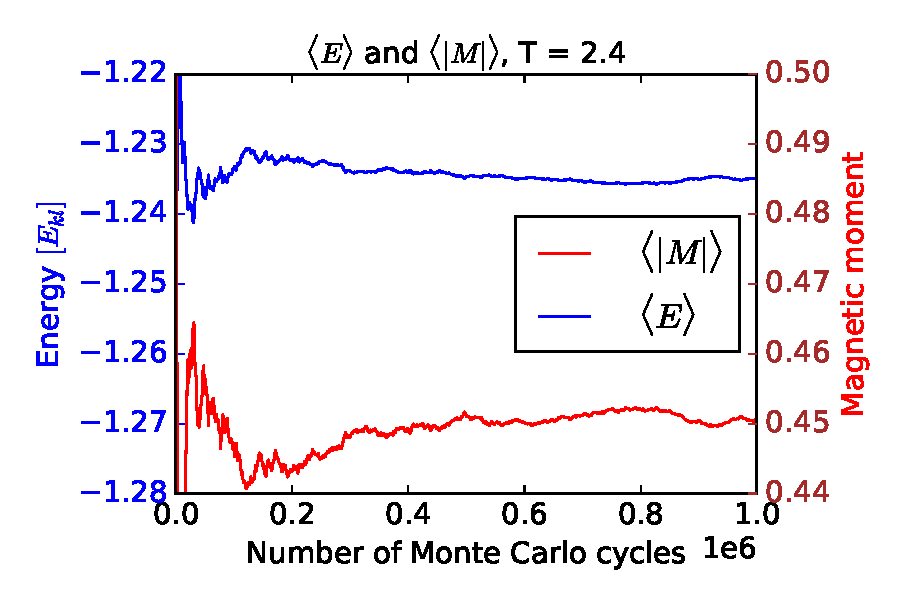
\includegraphics[width=\linewidth]{../results/4c/En_mag_T2_4}\caption{This is a plot of both the expectation value of the energy and absolute magnetic moment per spin verus number of Monte Carlo cycles at T = 2.4 K. The plot shows that an equilibrium is reached at around $5 \cdot 10^{5}$ MC cycles.}\label{fig:L_20_energy_mag_T_2.4}
\end{figure}

\subsubsection{Initial state}

\begin{figure}[H]
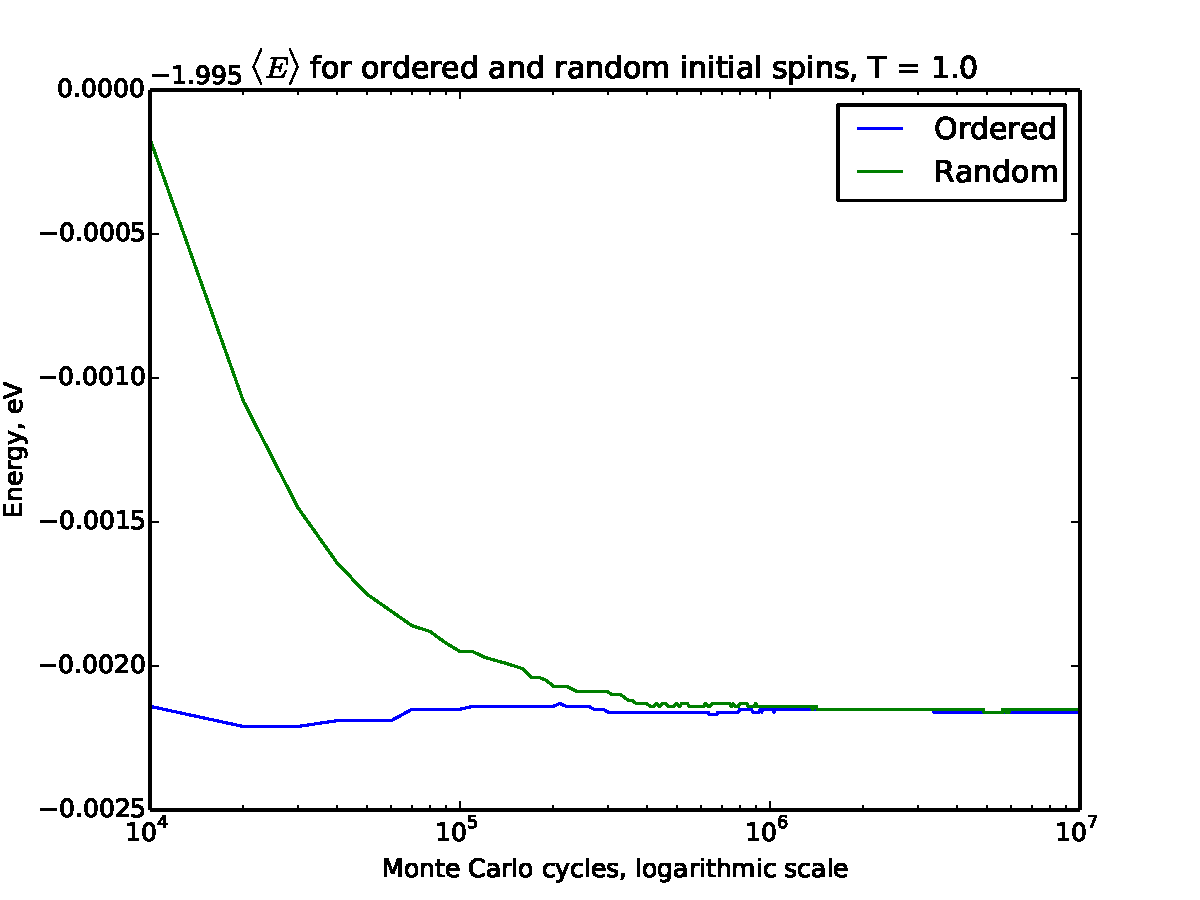
\includegraphics[width=\linewidth]{../results/4c/ran_order_T1}\caption{This is a plot of both the expectation value of the energy and absolute magnetic moment per spin verus number of Monte Carlo cycles at T = 1.0 K. The plot shows the difference in the behaviour of the ordered initial state and a random initial state.}\label{fig:L_20_initial_T_1.0}
\end{figure}

\begin{figure}[H]
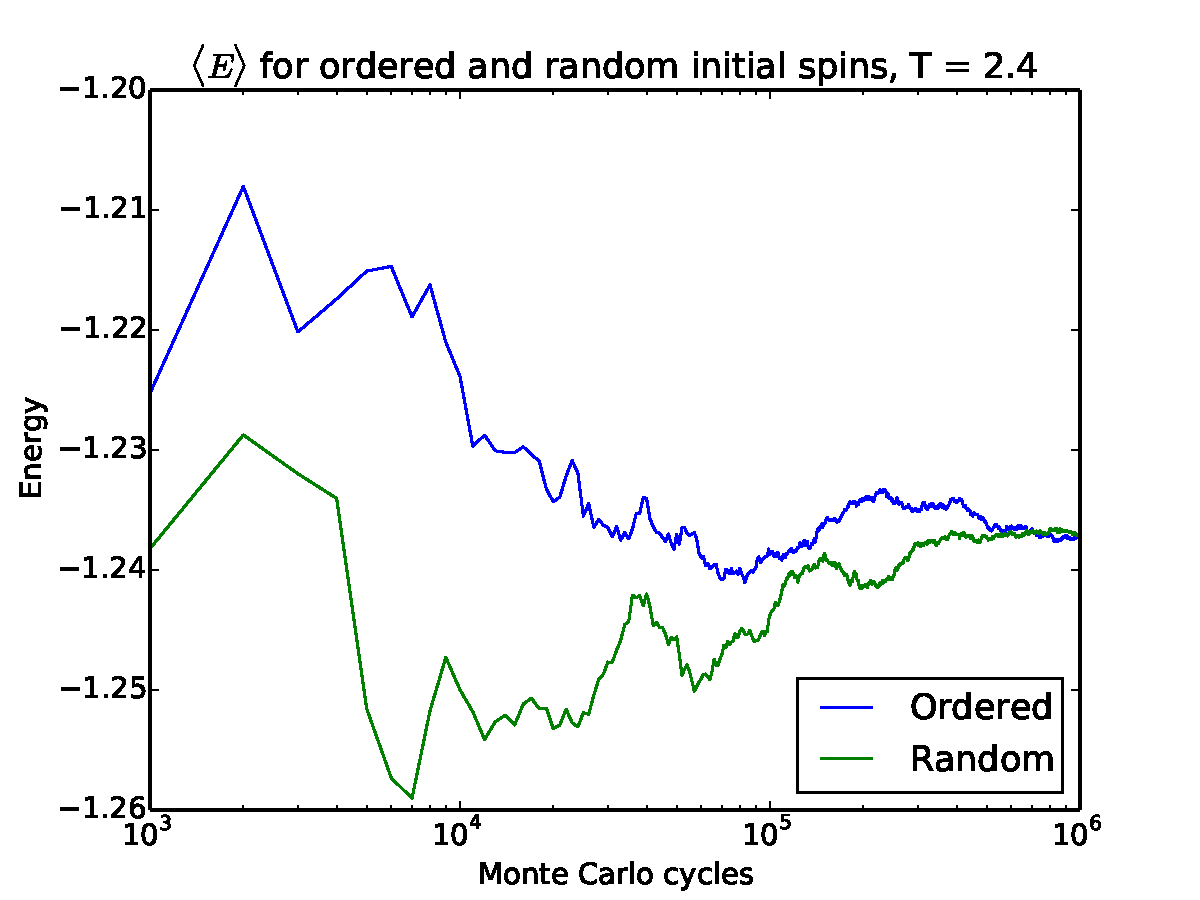
\includegraphics[width=\linewidth]{../results/4c/ran_order_T2}\caption{This is a plot of both the expectation value of the energy and absolute magnetic moment per spin verus number of Monte Carlo cycles at T = 2.4 K. The plot shows the difference in the behaviour of the ordered initial state and a random initial state.}\label{fig:L_20_initial_T_2.4}
\end{figure}

\subsubsection{Accepted configurations}

\begin{figure}[H]
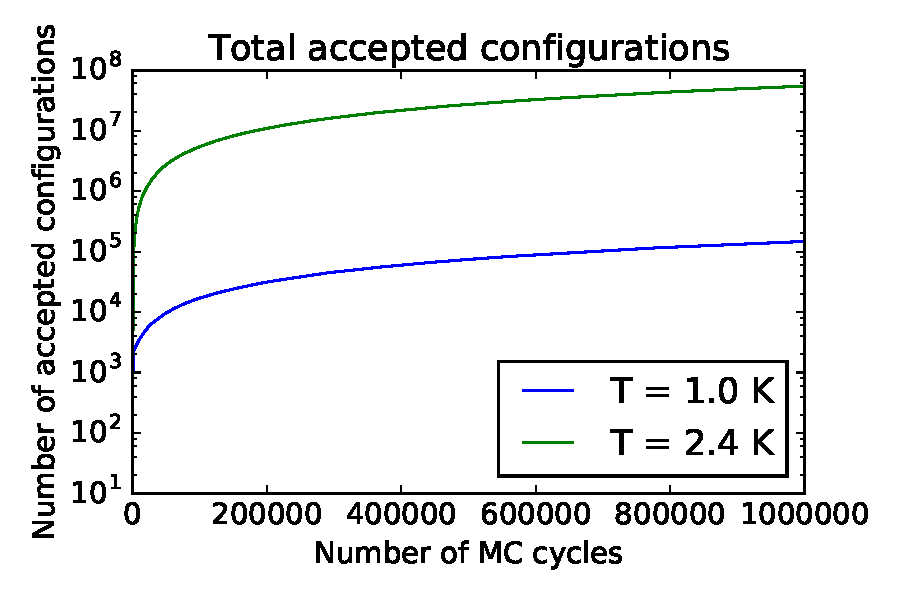
\includegraphics[width=\linewidth]{../results/4c/L_20_total_accepted}\caption{This is a plot of the total number of accepted configurations versus number of Monte Carlo cycles with random initial state.}\label{fig:total_accepted}
\end{figure}

\begin{figure}[H]
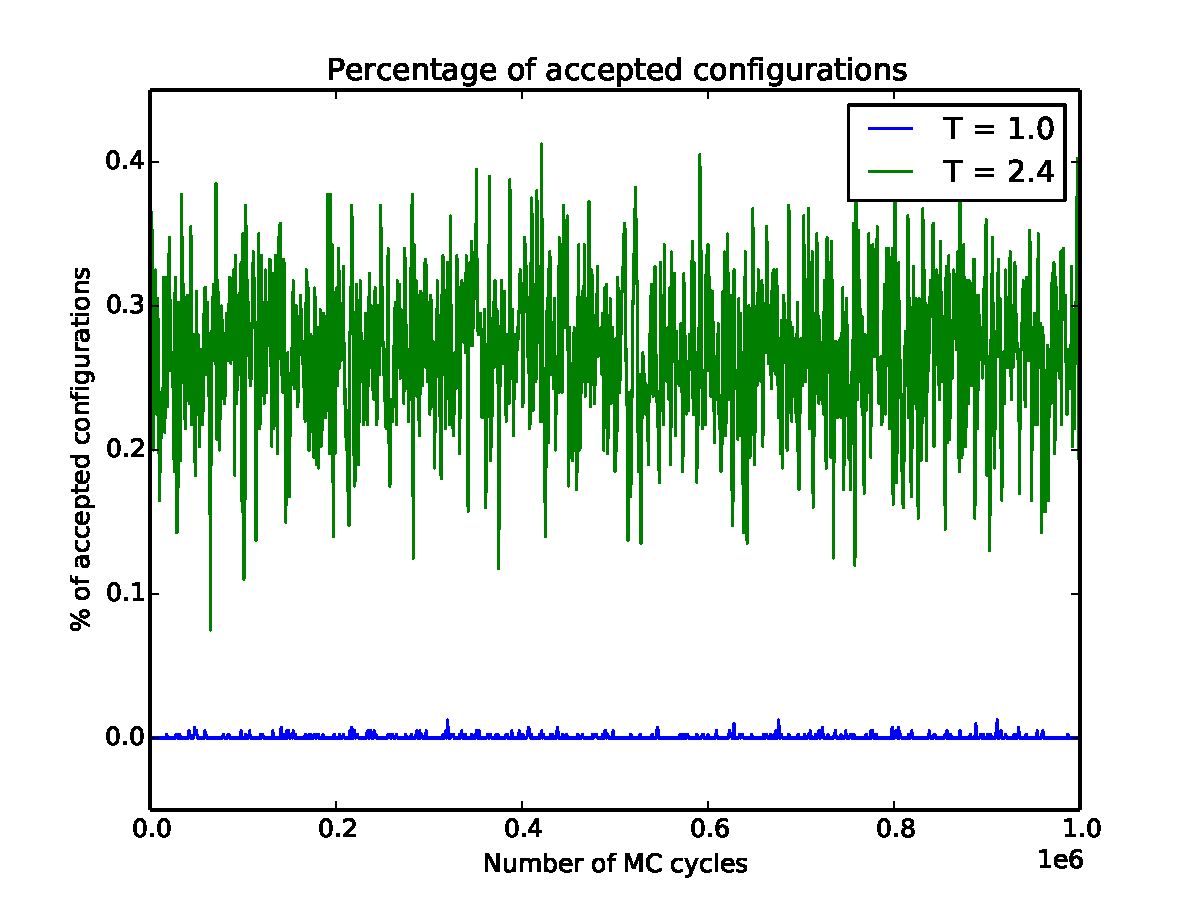
\includegraphics[width=\linewidth]{../results/4c/L_20_accepted_configs}\caption{This is a plot of the percentage accepted of attempted configurations versus  Monte Carlo cycles with random initial state.}\label{fig:percentage_accepted}
\end{figure}

\subsection{Energy probability}

OBS: Compare result with computed variance!

OBS: Discuss behavior (In Discussion - maybe just merge result and discussion?)

Computed variance (from same dataset?):

$$ \sigma_E^2 = \left< E^2\right> - \left< E\right>^2 $$
$$\text{FWHM} = 2 \sqrt{2ln2} \sigma \approx 2.355 \sigma$$ 

T = 1.0 K:
$$ \sigma_E^2 = 638181 - (-798.855)^2 = 11.69 $$
$$ \sigma = 3.42 $$
$$ \text{FWHM} \approx 2.355 \cdot 3.24 = 7.63 $$

T = 2.4 K:
$$ \sigma_E^2 =   247886 - (-494.628)^2 = 3229.14 $$
$$ \sigma = 56.8  $$
$$ \text{FWHM} \approx 2.355 \cdot 56.8 = 133.76 $$

\begin{figure}[H]
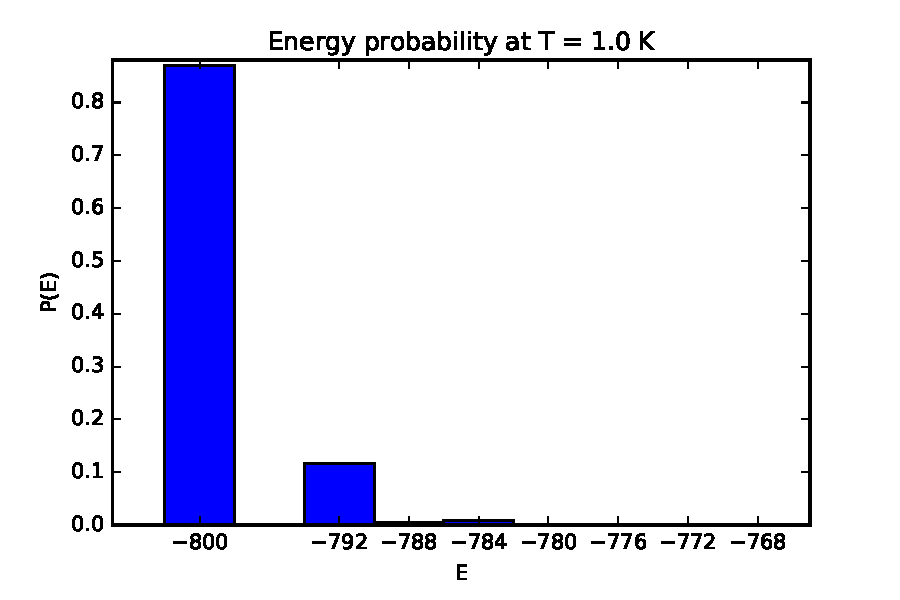
\includegraphics[width=\linewidth]{../results/4d/d_T_1probability}\caption{This is a plot of the energy probability when T = 1.0 K. The energy is the total energy of the 2D lattice with $20\times 20$ spins.}\label{fig:probability_T_1.0}
\end{figure}

\begin{figure}[H]
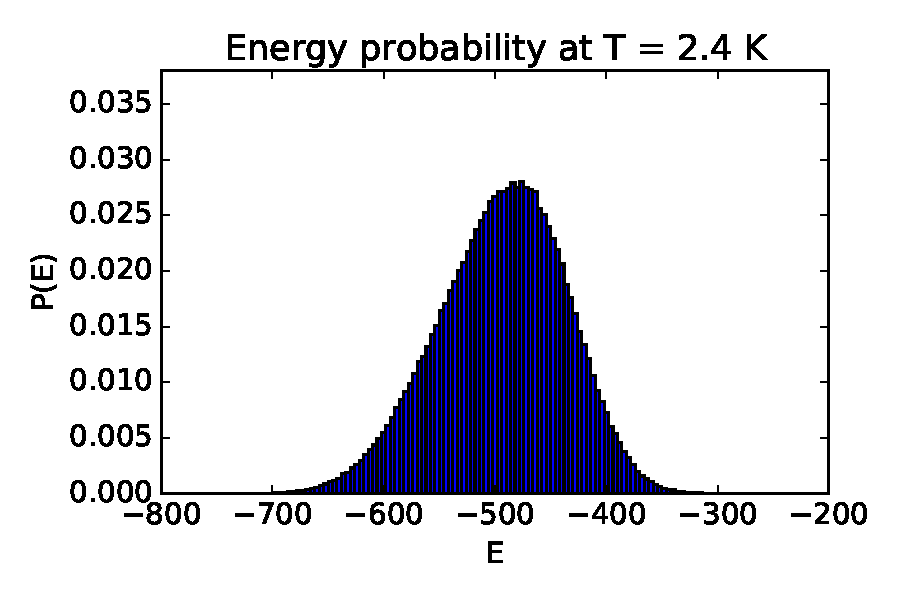
\includegraphics[width=\linewidth]{../results/4d/d_T_2_4probability}\caption{This is a plot of the energy probability when T = 2.4 K.The energy is the total energy of the 2D lattice with $20\times 20$ spins.}\label{fig:probability_T_2.4}
\end{figure}

\subsection{Increasing dimensionality/ Critical temperature}

\begin{figure}[H]
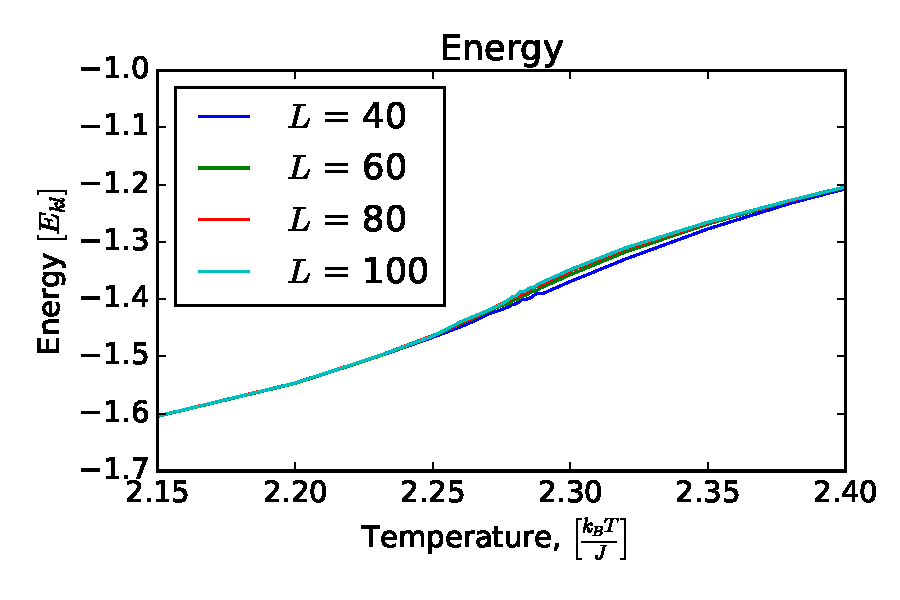
\includegraphics[width=\linewidth]{../results/4e/4e_energy}\caption{This is a plot if the energy versus temperature around the critical temperature for the different lattice sizes with L = 40, L = 60, L = 80 and L = 100.}\label{fig:4e_energy}
\end{figure}

\begin{figure}[H]
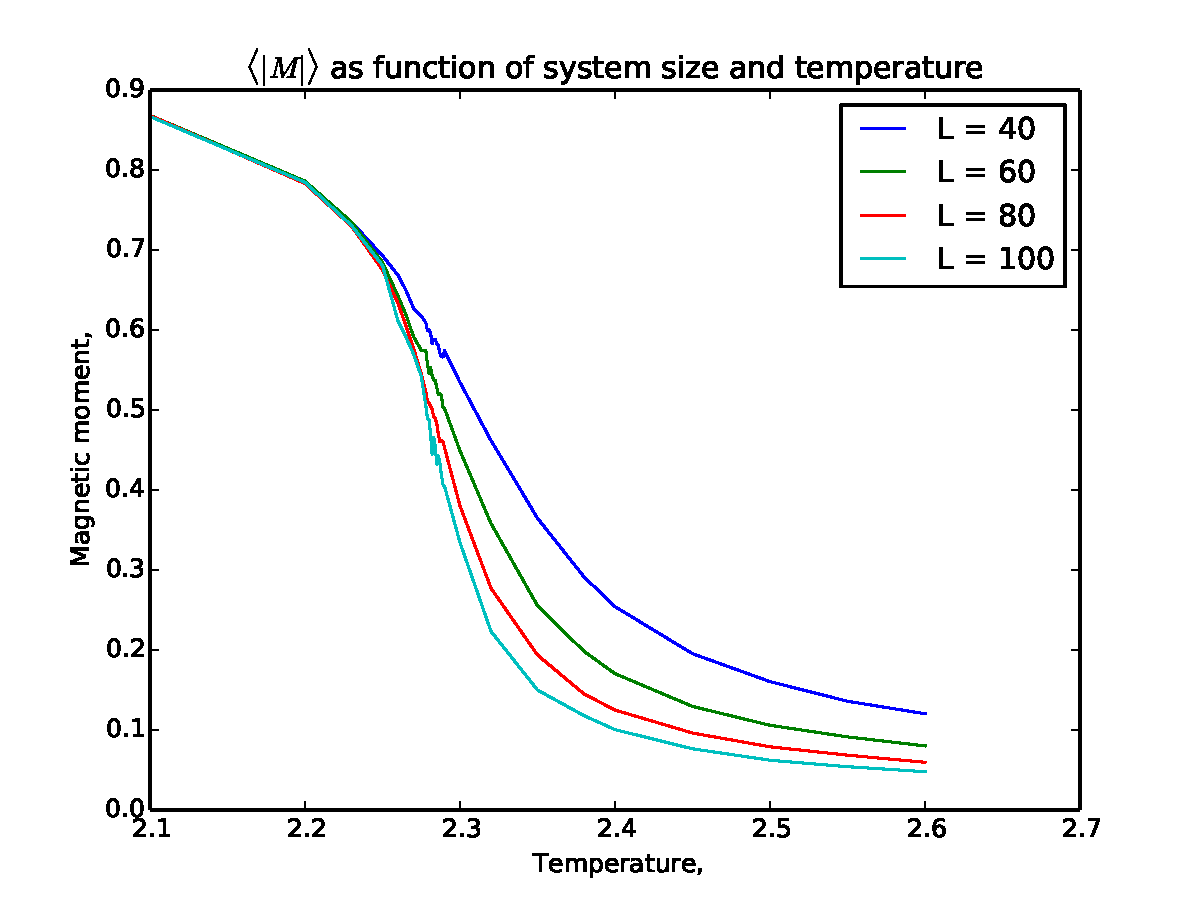
\includegraphics[width=\linewidth]{../results/4e/4e_mag}\caption{This is a plot if the absolute magnetic moment versus temperature around the critical temperature for the different lattice sizes with L = 40, L = 60, L = 80 and L = 100.}\label{fig:4e_magnetic}
\end{figure}

\begin{figure}[H]
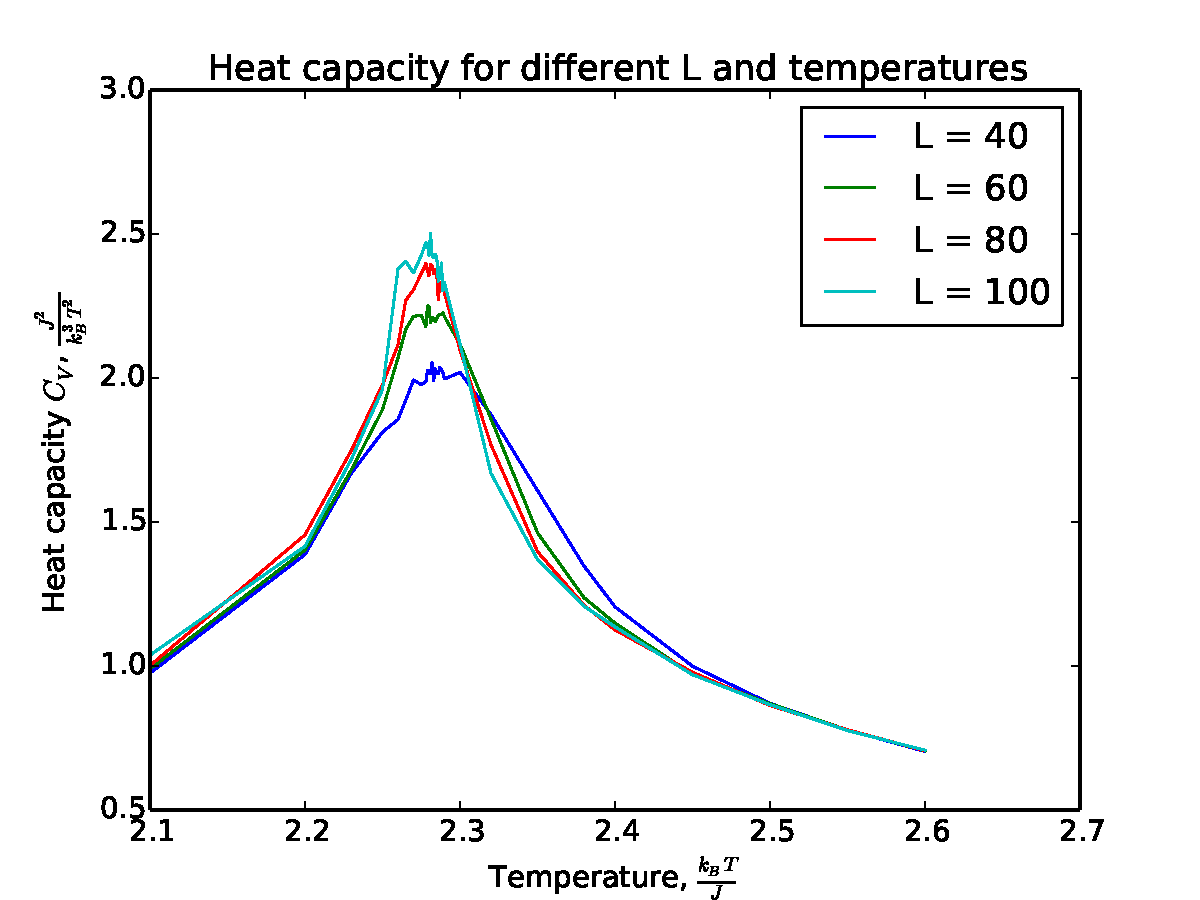
\includegraphics[width=\linewidth]{../results/4e/4e_Cv}\caption{This is a plot if the heat capacity versus temperature around the critical temperature for the different lattice sizes with L = 40, L = 60, L = 80 and L = 100.}\label{fig:4e_heat_capa}
\end{figure}

\begin{figure}[H]
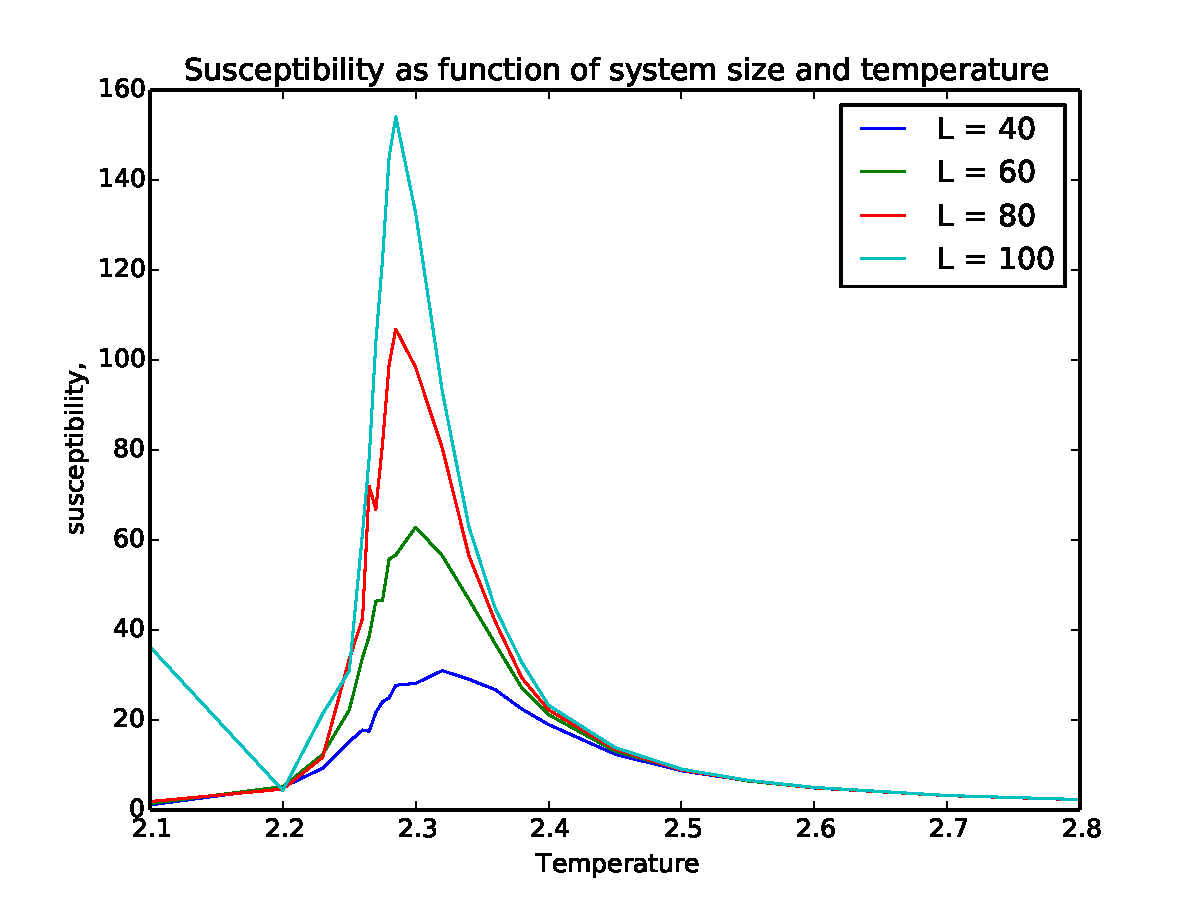
\includegraphics[width=\linewidth]{../results/4e/4e_x}\caption{This is a plot if the susceptibility versus temperature around the critical temperature for the different lattice sizes with L = 40, L = 60, L = 80 and L = 100. The exact value is $T_C =  kTC/J = 2/ \ln(1+\sqrt{
2}) \approx 2.269 \,\text{k}_\text{B} \,\text{K}$ \cite{Onsager}.}\label{fig:4e_suscept}
\end{figure}

OBS: Indication of phase transition? (Peak - at least for Cv and X)

OBS: Compare behaviour with equations?

OBS: Use Equation \ref{eq:critical_T} to extract $T_C$.

Getting these equations from \ref{eq:critical_T} where $\nu = 1$:
\begin{align*}
T_C(40) - T_C(\infty) &= a \cdot 40^{-1}\\
T_C(60) - T_C(\infty) &= a \cdot 60^{-1}\\
T_C(80) - T_C(\infty) &= a \cdot 80^{-1}\\
T_C(100) - T_C(\infty) &= a \cdot 100^{-1}\\
\end{align*}

(Sett inn tall!)
\begin{align}\label{eq:find_critial_T}
T_C(\infty) &= - a \cdot 40^{-1} + 2.28\\
T_C(\infty) &= - a \cdot 60^{-1} + 2.27\\
T_C(\infty) &= - a \cdot 80^{-1} + 2.28\\
T_C(\infty) &= - a \cdot 100^{-1} + 2.27\label{eq:find_critial_T_end}
\end{align}

\begin{figure}[H]
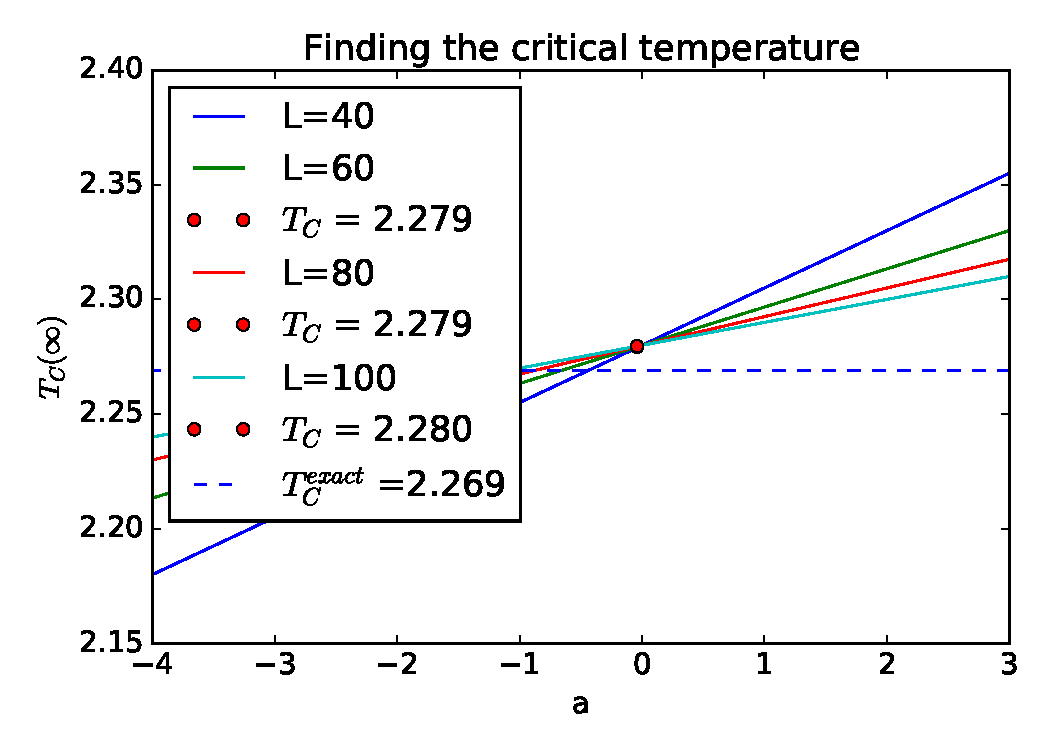
\includegraphics[width=\linewidth]{../results/4f/critical_t}\caption{This is a plot of Equation \ref{eq:critical_T} with different values of L (See Equations \ref{eq:find_critial_T} - \ref{eq:find_critial_T_end}). The interssections represent the solution. They should have all had a cross section in the same place, and the y-value of the intersection would have been the critical temperature when $L \rightarrow \infty$.}\label{fig:critical_T}
\end{figure}

Exact $T_C =  kTC/J = 2/ \ln(1+\sqrt{
2}) \approx 2.269$ \cite{Onsager}

\begin{table}\caption{L=60 and MC cycles is 1e6.}
\begin{tabular}{cc}
Number of processors:& CPU time [s]: \\ \hline
 1 & 513.069\\
 2 & 306.975\\
\end{tabular}
\end{table}